%chktex-file 1 %chktex-file 3 %chktex-file 8 %chktex-file 9 %chktex-file 10 %chktex-file 11 %chktex-file 12 %chktex-file 13 %chktex-file 16 %chktex-file 17 %chktex-file 18 %chktex-file 25 %chktex-file 26 %chktex-file 35 %chktex-file 36 %chktex-file 37 %chktex-file 40 %chktex-file 44 %chktex-file 45 %chktex-file 49
\section{Прямая сумма подпространств и пространств}
    \begin{definition}
        Сумма $U_1+...+U_m$ подпространств $U_i \subset V, \ 1\leq i \leq m$ называется прямой суммой, если 
        $\forall u \in U_1+...+U_m$  представим в виде: \\$u = u_1+...+u_m \ (u_i \in U_i)$  единственным образом    
    \end{definition} 
    Пусть $m=2, V$ - конечномерное пространство, $U_{1,2}$ - подпространства $V$
    \begin{theorem}
        Следующие условия равносильны: 
        \begin{enumerate}
            \item $U = U_1 + U_2$ - прямая сумма
            \item $U_1 \cap U_2 = \{0\}$
            \item $\dim (U_1 + U_2) = \dim U_1 + \dim U_2$
            \item Базис $U_1 + U_2$ - объединение базисов слагаемых    
        \end{enumerate} 
    \end{theorem} 
    \begin{proof}\tab
        \begin{itemize}
            \item[$1. \to 2.$] Допустим $v \in U_1 \cap U_2 \Longrightarrow v = \underset{\in U_1}{v} + 0 = 0 + \underset{\in U_2}{v}  \Longrightarrow v = 0$
            \item[$2. \to 3.$] По формуле Грассмана: 
            $$\dim (U_1 + U_2) = \dim U_1 + \dim U_2 - \underbrace{\dim (U_1 \cap U_2)}_{0}$$
            \item[$3. \to 4.$] Ввиду доказательства формулы Грассмана. Если $$\sum \limits_{i} \alpha_i a_i + \sum \limits_{j} \beta_j b_j = 0 \Longrightarrow \sum \limits_{i} \alpha_i a_i = \sum \limits_{j} (-\beta_j) b_j \in U_1 \cap U_2 = \{0\}$$
            $$\Longrightarrow  \text{все } \alpha_i \text{ и } \beta_i \text{ равны нулю}$$
            \item[$4. \to 1.$] $\forall u \in U_1 + U_2: $ $$
            u = (\sum \limits_{i} \alpha_i a_i) + (\sum \limits_{j} \beta_j b_j)$$ 
            - разложение по базису единственно  
        \end{itemize}
    \end{proof}
    \begin{theorem}
        Следующие условия равносильны: 
        \begin{enumerate}
            \item $U = U_1 + U_2 + ... + U_n$ - прямая сумма
            \item $\forall i, \ 1 \leq i \leq m, \ U_i \cap (\sum \limits_{j \neq i}U_j) = \{0\}$
            \item $\dim (U_1 + U_2 + ... + U_n) = \dim U_1 + \dim U_2 + ... + \dim U_n$
            \item Базис $U_1 + U_2 + ... + U_n$ - объединение базисов слагаемых    
        \end{enumerate} 
    \end{theorem}
    \begin{exercise}
        Доказать
    \end{exercise} 
    \begin{example1} того, что условия $U_i \cap U_j = \{0\}, \ i \neq j$ недостаточно для прямой суммы:
        \begin{center}
            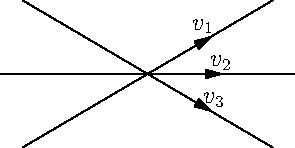
\includegraphics[width=5cm]{image/Asymptote/5/linal-5-1.pdf}
        \end{center}
    $v_1,v_2,v_3$ - ЛЗ $\Longrightarrow $ представление не единственным образом
    \end{example1}
    \begin{lemma}
        Любой ЛНЗ набор векторов $a_1,...,a_m$ в $n$-мерном векторном пространстве $V \ (m < n)$ можно дополнить до базиса в $V$.  
    \end{lemma}
    \begin{proof}
         \begin{enumerate}
            \item Пусть известны координаты векторов в некотором базисе $e_1,...,e_n \Longrightarrow rk \{a_1,...,a_m,e_1,...,e_n\} = n$
            \item Составим матрицу: 
            $$\begin{pmatrix}
                a_1^{\uparrow} & \cdots a_m^{\uparrow} & \vline & E_n
            \end{pmatrix} \xrightarrow[\text{выделяем базисные столбцы}]{\text{ЭП строк матрицы}} \begin{pmatrix}
            a_1^{\uparrow} & \cdots a_m^{\uparrow} & \vline & e_{i,1}^{\uparrow} & \vline & e_{j,n-m}^{\uparrow} & \cdots
            \end{pmatrix}$$
            Тогда к векторам $a_1,....,a_m$ надо добавить $e_{j,1},...,e_{j,n-m}$  
        \end{enumerate}
    \end{proof}
    \begin{definition}
        Если $U$ - подпр-во в $V \ (0 \neq U \neq V)$ и $\exists \ W \subset V \ : \ V = U \oplus W$, то $W$ - прямое дополнение к $U$.    
    \end{definition}
    \begin{consequense}
        Для любого подпространства в конечномерном векторном пространстве $\exists \ $ прямые дополнения. 
    \end{consequense} 
    \begin{proof}
        $U = \langle a_1,...,a_m \rangle \Longrightarrow \exists \ a_{m+1},...,a_n \ : \ \langle a_1,...,a_n \rangle$ - базис в $V$, тогда $W = \langle a_{m+1},...,a_n \rangle$   
    \end{proof}
    \begin{definition}
        Пусть $V_1,...,V_k \ (k\geq 2)$ - векторы пространства над одним и тем же полем $\mathbb{F}$, тогда: 
        $$V = V_1 \times ... \times V_k = \{ (v_1,...,v_k) \ | \ v_i \in V_i, 1\leq i \leq k\} - \text{ внешняя прямая сумма}$$ 
        Обозначение: $\begin{smallmatrix}
        \oplus \\ \circ 
    \end{smallmatrix}$
    \end{definition} 
    \begin{remark}
        Внешнюю прямую сумму $V = V_1 \begin{smallmatrix}
            \oplus \\ \circ
        \end{smallmatrix} ... \begin{smallmatrix}
            \oplus \\ \circ
        \end{smallmatrix} V_k$  можно превратить в прямую сумму подпространства:
        $$\forall i \text{ рассмотрим } V'_i = \{0,...,.v_i,....,0\} - \text{ подпространство в } V$$
        Запись $v_1,...,v_k \overset{\text{единственно}}{=} (v_1,0,0,...,0) + (0,v_2,0,...,0)+...+(0,0,0,...,v_k)$ показывает, что $V = V'_1 \oplus ... \oplus V'_k$ - единственно. \\
        В частности $\dim (V_1 \begin{smallmatrix}
            \oplus \\ \circ 
        \end{smallmatrix} ... \begin{smallmatrix}
            \oplus \\ \circ 
        \end{smallmatrix} V_k ) = \sum \limits_{i=1}^n \dim V_i$ 
    \end{remark} 
    \subsection*{Факторпространства}
    \begin{definition}
        Пусть $U \subset V$ - подпространство, $v_1,v_2 \in V$. Говорят, что $v_1 \thicksim v_2$ по модулю $U$, если $v_1 - v_2 \in U \ $. Классы эквивалентности имеют вид: 
        $$v + U = \{v + u \ | \ u \in U\}$$
        - смежные классы по $U$, где $v$ - представитель\\
        $*$ $V/U = \{\underbrace{v + U}_{\overline{v}}  \ | \ u \in U\}$
    \end{definition}
    \begin{subtheorem}
        $v_1 \thicksim  v_2 \Leftrightarrow v_1 + U = v_2 + U$
    \end{subtheorem}
    \begin{proof} \tab
        \begin{itemize}
            \item[$\underline{\Rightarrow} :$] Если $v_1 \thicksim v_2$, то $\exists \ u_0 \in V: v_2 = v_1 + u_0$
            $$\forall u \in U \ \ v_2 + u = v_1 + (u_0 + u) \Longrightarrow  v_2 + U \subseteq v_1 + U$$
            $$v_1 = v_2 - u_0; \ \forall u \in U \ v_1 + u = v_2 + (u - u_0) \Longrightarrow  v_1 + U \subseteq v_2 + U$$
            \item[$\underline{\Leftarrow} :$] Если $v_1 + U = v_2 + U$, то $\exists u_1 \in U: \ v_1 = v_2 + u_1 \Longrightarrow v_1 - v_2 = u_1 \in U$
        \end{itemize}
    \end{proof}
    \begin{definition}
        $v + U$ - смежный класс элемента $v$ по $U$ \ : \ $\bar{v} := v + U$
    \end{definition} 
    \begin{definition}
        $V / U = \{\bar{v} \ | \ v\in V\}$ - факторпространство $V$ по $U$.
    \end{definition} 
    \begin{definition}
        Структура векторного пространства на $V / U$:
        $$\overline{v}_1 + \overline{v}_2 = \overline{v_1 + v_2}; \ \ \ \lambda\overline{v}_1 = \overline{\lambda v_1};$$
    \end{definition} 
    \begin{definition}
        $\dim (V/U)$ называется коразмерностью подпространства $U$ в $V$ \\
        Обозначается: $\textup{Codim}_{V} U$ 
    \end{definition} 
    \begin{example1}
        Пусть $V = C[a, b]$ 
        $$U = \{f(x) \ | \ f(x_0) = 0, \ x_0 \in [a, b]\} \Longrightarrow \textup{Codim}_{V} U = 1$$
    \end{example1}
    \begin{theorem} \tab
        \begin{enumerate}
            \item Данные операции задают на $V/U$ векторное пр-во;
            \item Если $\dim V < \infty$, то $\dim(V/U) = \dim V - \dim U$
        \end{enumerate}
    \end{theorem}
    \begin{proof} \tab
        \begin{itemize}
            \item[$1)$] Проверим корректность введённых операций:\\
            Если $v'_1 = v_1 + u_1, \ v'_2 = v_2 + u_2, \ u_1, u_2\in U: $ 
            $$v'_1 + v'_2 = v_1 + v_2 + (u_1 + u_2)$$
            $$ v'_1 + v'_2 \sim v_1 + v_2, \text{ т.е. } v'_1 + v'_2 + U = v_1 + v_2 + U \Rightarrow \overline{v'_1 + v'_2} = \overline{v_1 + v_2}$$
            $$\overline{v'_1} + \overline{v'_2} = \overline{v'_1 + v'_2} = \overline{v_1 + v_2} = \overline{v_1} + \overline{v_2}$$
            т.е. сложение не зависит от выбора элементов в классах.\\
            Если 
            $$v' = v + u, \ u \in U \Longrightarrow \lambda v' = \lambda v + \lambda u \in \lambda v + U$$ 
            $$v \sim v' \Longrightarrow \lambda v \sim \lambda v'; \ \overline{0} \in U; \  -\overline{v} = \overline{-v}$$
            Все аксиомы выполенены, т.к. действия над смежными классами выражаются через действия над векторами.
            \item[$2)$] Выберем базис $a_1,...,a_m$ в $U$\\
            Если $U=V$, т.е. $m=n=\dim V$, то $V/U = \{0\} \Longrightarrow \dim (V/U) = n-n=0$\\
            Если же $m<n$, то можно дополнить базис $U$ векторами $a_{m+1},....,a_n$ до базиса в $V$, тогда классы $\overline{a_{m+1}},....,\overline{a_n}$ образуют базис в $V/U$ :
            $$\forall v \in V \ : \ v = \sum \limits_{i=1}^m \alpha_i a_i + \sum \limits_{j=m+1}^n \alpha_j a_j$$
            $$\overline{v} = v+ U = \sum \limits_{j=m+1}^n \overline{\alpha_j a_j} = \sum \limits_{j=m+1}^n \alpha_j \overline{ a_j}$$
            $\Longrightarrow \overline{a_{m+1}},....,\overline{a_n}$ порождают $V/U$\\
            Проверим ЛНЗ: 
            $$\exists \ \lambda_j \in \mathbb{F} \ : \ \sum \limits_{j=m+1}^n \lambda_j \overline{ a_j} = \overline{0} \Longleftrightarrow  \sum \limits_{j=m+1}^n \lambda_j a_j \in U$$
            $$\exists \ \mu_i \in \mathbb{F} \ : \ \sum \limits_{j=m+1}^n \alpha_j a_j - \sum \limits_{i=1}^m \mu_i a_i = 0$$
            Т.к. $\{a_1,...,a_n\}$ ЛНЗ, то $\lambda_j =0, \ \mu_i =0 , \ \forall i,j \Longrightarrow \overline{a_{m+1}},....,\overline{a_n}$ - ЛНЗ   
        \end{itemize}
    \end{proof}